% !TEX root = ../waves.tex
%%%%%%%%%%%%%%%%%%%%%%%%%%%%%%%%%%%%%%%%%%%%%%%%%%%%%%%%%%%%%%%%%%%%%%%%%%%%%%%%%%%%%%%%%%
As an introduction, we study a physical system which had a significant importance in the
historical development of Fourier analysis: the \emph{plucked string}. We consider in a
two-dimensional space a uniform string of length $L$ with linear mass density $\mu$ (in
$\kilogram\per\meter$), stretched between two points with coordinates $(0,0)$ and $(L,0)$.
We assume the string tension to be given by $T$ (in $\newton$). The action of plucking the
string consists in pulling it in a given position at time $t=0$, and releasing it. The
whole system is illustrated in~\cref{fig:string}. In the most general case, such system
can have a very complex behaviour, however we can introduce extra assumptions to simplify
it. We will assume in this section that we want to describe string vibrations for a
musical instrument, \eg an acoustic guitar. In this context, we clearly expect the string
oscillation to have an amplitude much smaller than the string length $L$.
\begin{figure}[t]
  \centering
  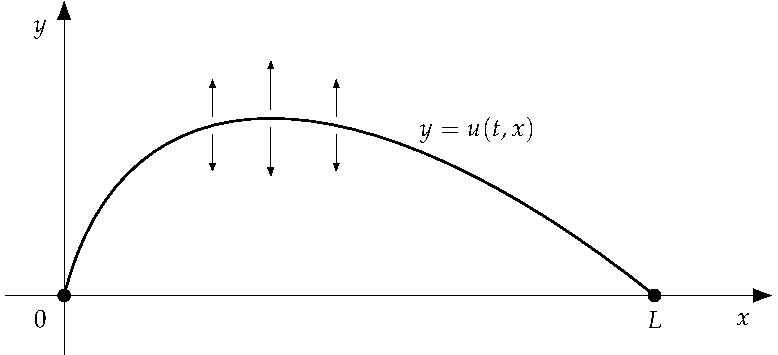
\includegraphics{tikz_string.pdf}
  \caption{Representation of the stretched string system. The arrows represent the
  transverse motion of the string.}
  \label{fig:string}
\end{figure}
%%%%%%%%%%%%%%%%%%%%%%%%%%%%%%%%%%%%%%%%%%%%%%%%%%%%%%%%%%%%%%%%%%%%%%%%%%%%%%%%%%%%%%%%%%
\section{Derivation of the wave equation}
Let us apply the laws of mechanics to derive an equation describing the dynamics of this
system. We first start by approximating the string by a large number $N$ of elastic line
segments of equal mass $\epsilon\mu$, with $\epsilon=\frac{L}{N}$. The $n$-th segment on
the string has the end points $P_n=(x_n,y_n)$ and $P_{n+1}=(x_{n+1},y_{n+1})$, starting
from $P_0=(0,0)$ up to $P_N=(L,0)$. The continuous string dynamics will then be later
obtained through the $N\to+\infty$ limit, or equivalently $\epsilon\to 0$. We additionally
assume that each segment respond to the same tension $T$ at its end points. A view of the
vicinity of $n$-th segment is represented in~\cref{fig:string-inf}. We define the angle
$\theta_n$ between the $n$-th segment and the $x$-axis. At the point $P_n$, the total
force $\vv{F}_n$ is given by the tension forces from the neighbouring segments on the
string, explicitly
\begin{equation}
  \vv{F}_n=\vv{T}_n^-+\vv{T}_n^+\,,\label{eq:string-force}
\end{equation}
where the vectors $\vv{T}_n^\pm$ both have magnitude $T$ and are represented by the
blue arrows in~\cref{fig:string-inf}. Using the angles $\theta_n$ previously defined, the
coordinates of the tension forces are given by
\begin{align}
  \vv{T}_n^-&=-T(\cos(\theta_{n-1}),\sin(\theta_{n-1}))\,,\\
  \vv{T}_n^+&=T(\cos(\theta_{n}),\sin(\theta_{n}))\,.
\end{align}
Using Pythagoras' theorem and elementary trigonometry, one can write
\begin{align}
  \cos(\theta_n)&=\frac{x_{n+1}-x_n}{\sqrt{(x_{n+1}-x_n)^2+(y_{n+1}-y_n)^2}}\,,\\
  \sin(\theta_n)&=\frac{y_{n+1}-y_n}{\sqrt{(x_{n+1}-x_n)^2+(y_{n+1}-y_n)^2}}\,.
\end{align}
Defining the ratio $d_n=\smash{\frac{y_{n+1}-y_n}{x_{n+1}-x_n}}$, the expressions above
can be further simplified to
\begin{equation}
  \cos(\theta_n)=\frac{1}{\sqrt{1+d_n^2}}\qquad\text{and}\qquad
  \sin(\theta_n)=\frac{d_n}{\sqrt{1+d_n^2}}\,.
\end{equation}
Now, using Newton's Second Law with the total force~\cref{eq:string-force}, one obtains
the following system of differential of equations for the motion of $P_n$:
\begin{align}
  \epsilon\mu \frac{\diff^2 x_n}{\diff t^2}&=
  T\left(\frac{1}{\sqrt{1+d_{\smash{n+1}}^2}}-\frac{1}{\sqrt{1+d_{n}^2}}\right)\,,
  \label{eq:string-fullxeq}\\
  \epsilon\mu \frac{\diff^2 y_n}{\diff t^2}&=
  T\left(\frac{d_{n+1}}{\sqrt{1+d_{\smash{n+1}}^2}}-\frac{d_n}{\sqrt{1+d_{n}^2}}\right)\,.
  \label{eq:string-fullyeq}
\end{align}
This is a rather non-trivial system of coupled non-linear differential equations, and we
will now use our small amplitude assumption to simplify it. This approximation means that
the vertical distances $y_{n+1}-y_n$ are expected to be much smaller than the horizontal
ones $x_{n+1}-x_n$, or in other words, $d_n$ is close to zero. Let us then
expand~\cref{eq:string-fullxeq,eq:string-fullyeq} for $d_n\to 0$. We first remind the
Taylor expansion
\begin{equation}
  \frac{1}{\sqrt{1+x^2}}=1-\frac{x^2}{2}+\mathcal{O}(x^4)\,,
\end{equation}
leading to the leading-order approximation
\begin{align}
  \frac{\diff^2 x_n}{\diff t^2}&=0\,,\label{eq:string-loxeq}\\
  \frac{\diff^2 y_n}{\diff t^2}&=\frac{T}{\epsilon\mu}(d_{n+1}-d_n)\,,\label{eq:string-loyeq}
\end{align}
which is valid up to $\mathcal{O}(d_n^2)$ corrections. One remarkable feature of this
system is the fact that there is no force applying in the $x$ direction at leading order.
Since we assumed the string to be attached at its end points, this implies that there is
no motion in the $x$ direction. Oscillations in the $x$ and $y$ directions are called
\emph{longitudinal} and \emph{transverse} oscillations, respectively. We just obtained a
well-known result for string oscillations: in the limit of small oscillations, only
transverse oscillations are present.
\begin{figure}[t]
  \centering
  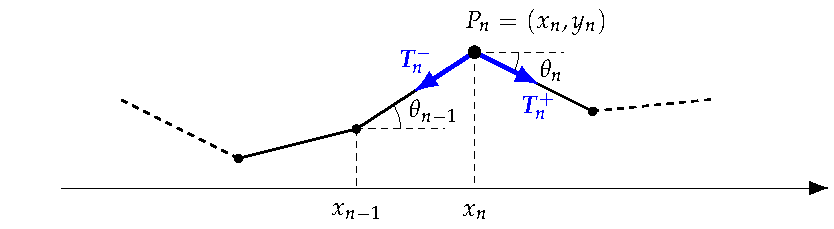
\includegraphics{tikz_string-inf.pdf}
  \caption{Discrete view of the string geometry and forces. The blue arrows represent the
  individual tension forces at point $P_n$.}
  \label{fig:string-inf}
\end{figure}

With the observation above, we can now exclusively focus on solving the transverse
equation of motion~\cref{eq:string-loyeq}. We assumed the string to have a uniform mass
distribution, and since the $x_n$ coordinates are constant and divide the string in
segments of equal mass, for all $n$ one has
\begin{equation}
  x_{n+1}-x_n=\epsilon\,.
\end{equation}
We additionally define the coordinates $y_n$ to be represented by a smooth function $u$ of
$x_n$ and the time $t$:
\begin{equation}
  y_n=u(t,x_n)\,.
\end{equation}
Substituting the equations above in~\cref{eq:string-loyeq}, one obtains
\begin{equation}
  \pdn{u}{t}{2}(t,x_n)=\frac{T}{\epsilon^2\mu}
  [u(t,x_{n}+\epsilon)-2u(t,x_{n})+u(t,x_{n}-\epsilon)]\,.\label{eq:wave-eq-discrete}
\end{equation}
We are now ready to obtain the continuous string equation by taking the $\epsilon\to 0$
limit. One starts by writing the Taylor expansion
\begin{equation}
  u(t,x+\epsilon)=u(t,x)+\epsilon\,\pd{u}{x}(t,x)
  +\frac{\epsilon^2}{2}\pdn{u}{x}{2}(t,x)+\mathcal{O}(\epsilon^3)\,,
\end{equation}
which implies that
\begin{equation}
  \lim_{\epsilon\to 0}=\frac{1}{\epsilon^2}
  [u(t,x+\epsilon)-2u(t,x)+u(t,x-\epsilon)]=\pdn{u}{x}{2}(t,x)\,.
\end{equation}
Using this last step with~\cref{eq:wave-eq-discrete} leads us to the main result of this
section, the \emph{wave equation}
\begin{equation}
  \boxed{
    \pdn{u}{t}{2}=c^2\,\pdn{u}{x}{2}
    \qquad\text{with}\qquad
  c=\sqrt{\frac{T}{\mu}}\,.}
  \label{eq:wave-eq}
\end{equation}
The parameter $c$, which has dimensions $\mathrm{L}\mathrm{T}^{-1}$, is usually called the
\emph{wave speed} for reasons that will be clear later in this section. The wave equation
is a homogeneous second-order partial differential equation, and will now discuss how to
solve it for the plucked string problem.
%%%%%%%%%%%%%%%%%%%%%%%%%%%%%%%%%%%%%%%%%%%%%%%%%%%%%%%%%%%%%%%%%%%%%%%%%%%%%%%%%%%%%%%%%%
\section{Travelling wave solutions}
\label{sec:wave-eq-travelling}
\subsection{General solutions}
We will first derive the general form of the solutions of the wave
equation~\cref{eq:wave-eq}. This derivation was first written by Jean le Rond d'Alembert
in 1747. \cref{eq:wave-eq} can be rewritten as follows
\begin{equation}
  \left(\pdn{}{t}{2}-c^2\,\pdn{}{x}{2}\right)u=
  \left(\pd{}{t}-c\,\pd{}{x}\right)
  \left(\pd{}{t}+c\,\pd{}{t}\right)u=0\,,
  \label{eq:wave-eq-factor}
\end{equation}
which is the composition of two first order derivatives. From this form, we would like to
define new length variables $\eta$ and $\xi$ such that
\begin{align}
  c\pd{}{\eta}&=\pd{}{t}+c\,\pd{}{x}\,,\\
  c\pd{}{\xi}&=\pd{}{t}-c\,\pd{}{x}\,.
\end{align}
Using the chain rule, we know that
\begin{align}
  \pd{}{\eta}&=\pd{t}{\eta}\pd{}{t}+\pd{x}{\eta}\pd{}{x}\,,\\
  \pd{}{\xi}&=\pd{t}{\xi}\pd{}{t}+\pd{x}{\xi}\pd{}{x}\,\,,
\end{align}
which implies that
\begin{equation}
  \pd{t}{\eta}=\frac{1}{c},\qquad\pd{x}{\eta}=1,\qquad
  \pd{t}{\xi}=\frac{1}{c},\qquad\text{and}\qquad\pd{x}{\xi}=-1\,.
\end{equation}
It is now clear that
\begin{align}
  t&=\frac{1}{c}(\eta+\xi)\,,\\
  x&=\eta-\xi\,,
\end{align}
is a possible solution, which can be inverted to
\begin{align}
  \eta&=x+ct\,,\\
  \xi&=x-ct\,.
\end{align}
In these new variables, the wave equation~\cref{eq:wave-eq-factor} becomes
\begin{equation}
  \frac{\partial^2 u}{\partial\eta\partial\xi}=0\,.
\end{equation}
In this simpler form, we can integrate the two derivatives sequentially. Starting with the
derivative in $\eta$, the right-hand side of the equation being zero means that
$\smash{\pd{u}{\xi}}$ is a constant in $\eta$. However, this constant can vary for any
value of $\xi$. In other words, there exists a function of one variable $\phi$ such that
\begin{equation}
  \pd{}{\xi}u(\eta,\xi)=\phi(\xi)\,.
\end{equation}
Following the same logic, as a function of $\xi$, $u$ is therefore an antiderivative of
$\phi$ up to a constant, which can vary with $\eta$. Therefore, there exists two functions
of a single variable $f$ and $g$ such that
\begin{equation}
  u(\eta,\xi)=f(\xi)+g(\eta)\,,
\end{equation}
where here $f$ is such that $f'=\phi$. In conclusion, switching back to the original
variables $x$ and $t$, the general solutions of the wave equation have the form
\begin{equation}
  \boxed{u(t,x)=f(x-ct)+g(x+ct)\,,}\label{eq:wave-eq-sol}
\end{equation}
where $f$ and $g$ can be any twice-differentiable functions. $f$ and $g$ are called the
\emph{forward-travelling} and \emph{backward-travelling} wave functions, respectively.
These functions are named in this way for the following reason. At $t=0$, if one pick a
point on the curve of $f$ with $x$-coordinate $x_0$, then at an arbitrary time $t$ the
same point will have the $x$-coordinate
\begin{equation}
  x(t)=x_0+ct\,,
\end{equation}
\ie it is moving forward on the $x$ axis. Also, one notices that $\td{x}{t}=c$, meaning
the point is moving with speed $c$, justifying the name \emph{wave speed} introduced
earlier. The same observation can be made for $g$, moving backward on the $x$ axis.

As we can see, the space of solutions of the wave equation is very large as both forward
and backward contribution are arbitrary functions. However, it is known, and will be
admitted here, that the wave equation has a unique solution if one impose the two initial
conditions
\begin{equation}
  u_0(x)=u(0,x)\qquad\text{and}\qquad u_1(x)=\pd{u}{t}(0,x)\,,\label{eq:wave-eq-ic}
\end{equation}
which physically represent the initial position of the string and its initial velocity,
respectively. With this in mind, we will now discuss the solution of the wave equations
specifically for the plucked string problem.
%
\subsection{Particular solutions of the plucked string problem}
We remind here the considered physical problem: the string will be pulled in a given
position, and then released. This means the initial velocity $u_1$ in~\cref{eq:wave-eq-ic}
is zero. Without specifying, for the moment, the initial position, let us discuss what
this first initial condition implies. Coming back to the general
solution~\cref{eq:wave-eq-sol}, $u_1=0$ implies that for all $x$,
\begin{equation}
  u_1(x)=c[g'(x)-f'(x)]=0\,,
\end{equation}
which means that $f'=g'$. Two functions with equal derivatives differ by a unique
constant, so there is a unique real number $K$ such that $g(x)=f(x)+K$ for all $x$. So the
general solution of the wave equation becomes
\begin{equation}
  u(t,x)=f(x-ct)+f(x+ct)+K\,,\label{eq:uff}
\end{equation}
and in particular the initial position is
\begin{equation}
  u_0(x)=2f(x)+K\,.\label{eq:u0K}
\end{equation}
Now, we can use the fact that the string is attached at the two points $(0,0)$ and
$(L,0)$, this implies that for all $t$
\begin{equation}
  u(t,0)=0\qquad\text{and}\qquad u(t,L)=0\,.\label{eq:string-bc}
\end{equation}
These constraints are called the \emph{boundary conditions} of the wave equation, and they
generally have a strong influence on the set of solutions. Applying the boundary
conditions at $t=0$ to~\cref{eq:u0K} directly implies that $K=0$, and also determines
$f(x)$ on the interval $[0,L]$:
\begin{equation}
  \forall x\in[0,L],\quad f(x)=\frac{1}{2}u_0(x)\,.
\end{equation}
However, the solution~\cref{eq:uff} requires us to know $f$ outside the interval $[0,L]$,
specifically for times $t>\frac{L}{c}$. At an arbitrary time $t$, the first boundary
condition in~\cref{eq:string-bc} becomes
\begin{equation}
  f(-ct)=-f(ct)\,,
\end{equation}
which means that the function $f$ is odd. In particular this tells us that for any
$x\in[-L,0]$, $f(x)=-f(-x)=-u_0(x)$. We now know the solution on the interval $[-L,L]$.
Repeating this exercise with the second condition in~\cref{eq:string-bc}, we get
\begin{equation}
  f(ct+L)=-f(L-ct)=f(ct-L)\,.
\end{equation}
Now, for any $x\in [-L,L]$, the previous equation evaluated at $t=\frac{1}{c}(x+L)$ gives
\begin{equation}
  f(x+2L)=f(x)\,,
\end{equation}
meaning that $f$ in the interval $[L,3L]$ is just a translation of its restriction to
$[-L,L]$. The argument above can be repeated multiple times to obtain
\begin{equation}
  f(x+2nL)=f(x)
\end{equation}
for any real number $x$ and integer $n$. This last equation means that $f$ is periodic
with period $\lambda=2L$, called the \emph{wavelength} of the vibration. We have now
completely and uniquely solved the wave equation for the plucked string problem, and we
summarise the solution below
\begin{equation}
  u(t,x)=f(x-ct)+f(x+ct)\,,\label{eq:string-sol}
\end{equation}
with
\begin{equation}
  f(x)=
  \begin{cases}
    u_0(x-2nL)&~\text{if}\quad2nL\leq x\leq (2n+1) L\\
    -u_0(2nL-x)&~\text{if}\quad(2n-1)L\leq x\leq 2nL
  \end{cases}
  \,,\label{eq:f-copies}
\end{equation}
where $n$ is any integer, and $u_0(x)$ is the initial string position. One important
observation can be made: since $f$ is periodic with period $\lambda$, it implies
using~\cref{eq:string-sol} that $u(t,x)$ is also periodic in time with period
\begin{equation}
  \tau=\frac{\lambda}{c}\,.
\end{equation}
Now, defining the \emph{frequency} $\smash{\omega=\frac{1}{\tau}}$, and reminding the
definition of $c$ from~\cref{eq:wave-eq}, we obtain
\begin{equation}
  \boxed{\omega=\frac{c}{\lambda}=\frac{1}{2L}\sqrt{\frac{T}{\mu}}}\,.
  \label{eq:mersenne-law}
\end{equation}
This result is called \emph{Mersenne's law}, and predicts the vibration frequency of a
string as a function of its length, tension, and linear mass density.

\begin{figure}[t]
  \centering
  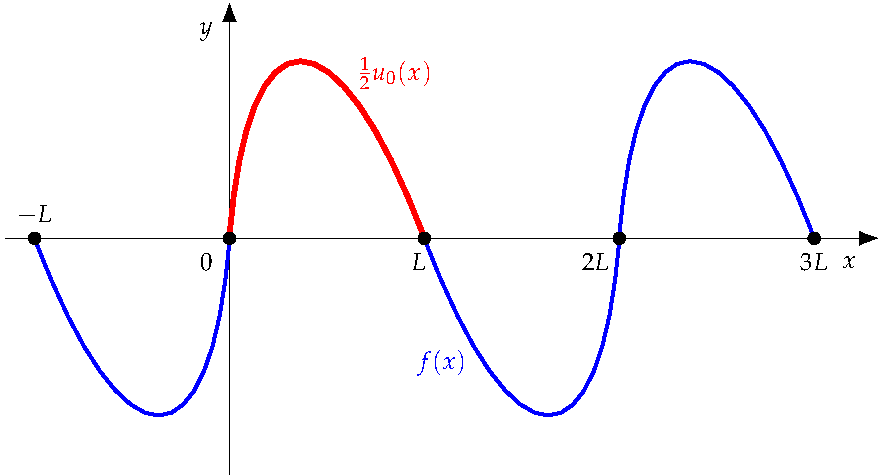
\includegraphics{tikz_string-f.pdf}
  \caption{Graphical representation of~\cref{eq:f-copies}. The bold red line represents
    the initial string position $u_0(x)$. The blue line is the forward component $f(x)$,
  obtained as the periodic extension of $u_0(x)$ defined in~\cref{eq:f-copies}.}
  \label{fig:string-f}
\end{figure}
\begin{figure}[t]
  \centering
  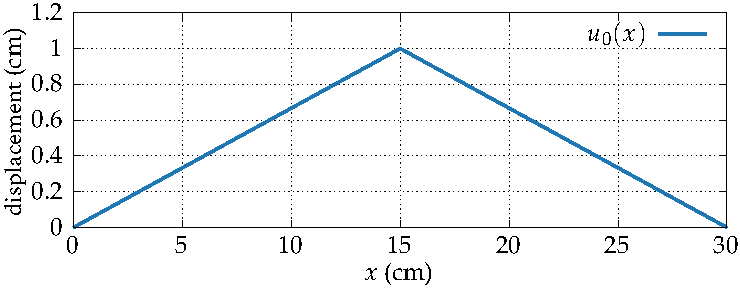
\includegraphics{gp_string-pulled.pdf}\\
  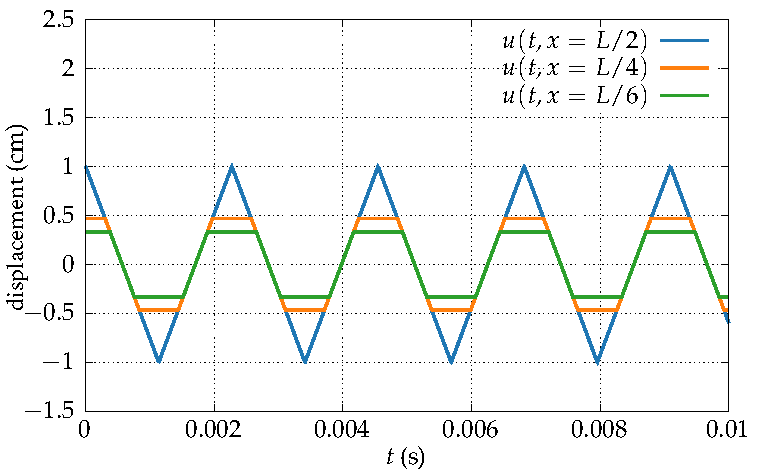
\includegraphics{gp_string-pulled-time.pdf}
  \caption{Initial condition~\cref{eq:string-pluck-ic} (upper pane) and resulting
    oscillations in time at various positions on the string (lower pane) with
    $A=\unit{1}{\centi\metre}$, $L=\unit{30}{\centi\metre}$, $T=\unit{63.4}{\newton}$, and
  $\mu=\unit{0.91}{\gram\per\metre}$.}
  \label{fig:string-pulled}
\end{figure}
We conclude this section by a slightly more practical discussion of the structure of the
solution. \cref{eq:f-copies} is somewhat abstract, but all it means is that the curve of
$f$ is constructed by sequentially repeating the curve of $u_0(x)$, rotating it by
$180^{\circ}$ at each iteration. This construction is illustrated in~\cref{fig:string-f}.
%
\subsection{Explicit example}
Let us now look at an explicit solution. We assume that initially the string middle point
is pulled to a distance $A$ from the $x$-axis, and that it is perfectly straight between
this point and its extremities. Explicitly, this can be parameterised by the following
initial condition
\begin{equation}
  u_0(x)=
  \begin{cases}
    \frac{2A}{L}x&~\text{if}\quad 0\leq x \leq \frac{L}{2}\\
    \frac{2A}{L}(L-x)&~\text{if}\quad \frac{L}{2}\leq x \leq L
  \end{cases}\,,
  \label{eq:string-pluck-ic}
\end{equation}
represented in the upper pane of~\cref{fig:string-pulled}. Let us give explicit values for
the all the parameters of the problem. We assume the string length $L$ is
$\unit{30}{\centi\metre}$, its linear mass density $\mu$ is
$\unit{0.91}{\gram\per\metre}$, and it is stretched to a tension $T$ of
$\unit{63.4}{\newton}$. We additionally assume the pulling distance $A$ to be
$\unit{1}{\centi\metre}$. Let us start by using~\cref{eq:wave-eq} to compute the wave
speed $c$
\begin{equation}
  c=\sqrt{\frac{T}{\mu}}
  =\sqrt{\frac{\unit{63.4}{\newton}}{\unit{0.91\times 10^{-3}}{\kilo\gram\per\metre}}}
  =\unit{263.95}{\metre\per\second}\,.
\end{equation}
Then, using Mersenne's law~\cref{eq:mersenne-law} with the wavelength
$\lambda=2L=\unit{60}{\centi\metre}$, we can compute the frequency of the string
vibration:
\begin{equation}
  \omega=\frac{c}{\lambda}=\frac{\unit{263.95}{\metre\per\second}}{\unit{0.6}{\metre}}
  =\unit{439.92}{\hertz}.
\end{equation}
So this string is approximately tuned to give the standard musical pitch $\mathrm{A}_4$ at
the $\unit{440}{\hertz}$ frequency. Explicit plots of the string vibrations at different
positions on the string are given in the lower pane of~\cref{fig:string-pulled}.
%%%%%%%%%%%%%%%%%%%%%%%%%%%%%%%%%%%%%%%%%%%%%%%%%%%%%%%%%%%%%%%%%%%%%%%%%%%%%%%%%%%%%%%%%%
\section{Standing wave solutions}
The previous steps entirely solved the wave equation for the problem we are interested in.
However, there is another way to solve this equation which is going to be very relevant
for what follows. Let us come back to~\cref{fig:string-f} and how the wave equation
forward wave function $f$ is built as a periodic extension of the initial condition. One
can notice how the symmetries of $f$, \ie it is periodic and odd, are identical to those
of the sine function. In fact, the structure of $f$ implies that if we would initially
pull the string into a position which is exactly half a period of the sine function, \ie
\begin{equation}
  \forall x\in[0,L],\quad u_0(x)=A\sin\left(\frac{\pi}{L}x\right)\,,\label{eq:string-sine-ic}
\end{equation}
then the extension~\cref{eq:f-copies} of $u_0$ to $f$ is defined by the same formula, \ie
$f(x)=\smash{A\sin\left(\frac{\pi}{L}x\right)}$ for any real number $x$, and the solution
to the wave equation is simply
\begin{equation}
  u(t,x)=\frac{A}{2}\left\{\sin\left[\frac{\pi}{L}(x+ct)\right]
  +\sin\left[\frac{\pi}{L}(x-ct)\right]\right\}\,.
\end{equation}
The choice~\cref{eq:string-sine-ic} is not unique, all is needed for the sine function is
to take the value zero at $x=0$ and $x=L$, which can generally be obtained with
\begin{equation}
  u_0(x)=A\sin\left(\frac{\pi}{L}nx\right)\,,
\end{equation}
where $n$ is an arbitrary integer, and the associated solution is
\begin{equation}
  u(t,x)=\frac{A}{2}\left\{\sin\left[\frac{\pi}{L}n(x+ct)\right]
  +\sin\left[\frac{\pi}{L}n(x-ct)\right]\right\}\,.
\end{equation}
Now, using the trigonometric identities
\begin{align}
  \sin(a+b)&=\sin(a)\cos(b)+\cos(a)\sin(b)\,,\\
  \sin(a-b)&=\sin(a)\cos(b)-\cos(a)\sin(b)\,,
\end{align}
$u(t,x)$ can be simplified to
\begin{equation}
  u(t,x)=A\sin\left(\frac{\pi}{L}nx\right)\cos\left(\frac{\pi}{L}nct\right)
  =\cos\left(\frac{\pi}{L}nct\right)f(x)\,.
  \label{eq:stand-wave-example}
\end{equation}
In this particular solution, time and space oscillations factorise and the wave function
$f$ does not ``travel'' any more. Such solution is called a \emph{standing wave solution}
of the wave equation. At this stage, this might just look like a special set of particular
solutions built on the symmetries of $f$. However, as we will see in this course, those
are of extreme importance for describing oscillatory phenomena, and were historically a
crucial part of the work of Jean-Baptiste Joseph Fourier (early 19\textsuperscript{th}
century), which led to the so-called Fourier analysis theory.

For now, let us question the generality of the standing wave solution above. To do that,
we start by considering a general standing wave solution of the wave equation:
\begin{equation}
  u(t,x)=F(t)G(x)\,.
\end{equation}
Applying the wave equation~\cref{eq:wave-eq}, one obtains
\begin{equation}
  \left(\pdn{}{t}{2}-c^2\,\pdn{}{x}{2}\right)u(t,x)=F''(t)G(x)-c^2F(t)G''(x)=0\,,
\end{equation}
which implies that
\begin{equation}
  \frac{F''(t)}{F(t)}=c^2\frac{G''(x)}{G(x)}\,.\label{eq:sep-var}
\end{equation}
The left-hand side of this equation only depends on $t$, and the right-hand side only
depends on $x$. This is typical of standing wave solution, and looking for such
simplification is sometime referred as the \emph{separation of variables} method, which in
this context is equivalent to looking for standing wave solutions. A key observation is
that~\cref{eq:sep-var} implies that there exists a constant $\alpha$ such that
\begin{equation}
  \frac{1}{c^2}\frac{F''(t)}{F(t)}=\frac{G''(x)}{G(x)}=\alpha\,.
\end{equation}
Indeed, since this expression can be written solely as a function of $x$ or $t$, it means
that both its partial derivatives in $x$ and $t$ vanish, implying that it is a constant
function of $x$ and $t$. With that established, the equation above can be rewritten as the
following system of ordinary differential equations
\begin{align}
  F''(t)&=c^2\alpha F(t)\,,\label{eq:sep-var-F}\\
  G''(x)&=\alpha G(x)\,.
\end{align}
We can solve these equations using the \emph{characteristic equation method}. Let us start
with the equation for $G$. We try to look for particular solutions of the form
\begin{equation}
  G(x)=e^{rt}\,,
\end{equation}
which would imply that
\begin{equation}
  G''(x)=r^2e^{rx}=\alpha e^{rx}\,,
\end{equation}
and therefore for such solution to exists $A$ must be a solution of the characteristic
equation
\begin{equation}
  r^2-\alpha=0\,.
\end{equation}
At this stage $\alpha$ is an arbitrary real number, and depending on its sign the equation
above can have the different solutions. For convenience let us define
$\beta=\smash{\sqrt{|\alpha|}}$, we have the following cases
\begin{enumerate}
  \item $\alpha>0$: then $r$ is a real number equal to $\pm \beta$, the particular
    solutions for $G(x)$ are $\smash{e^{\beta x}}$ and $\smash{e^{-\beta x}}$, and the
    general solutions are the linear combinations $G(x)=a\smash{e^{\beta
    x}}+b\smash{e^{-\beta x}}$ for any real numbers $a$ and $b$.
  \item $\alpha<0$: then $r$ is a purely imaginary complex number equal to $\pm i\beta$,
    the particular solutions for $G(x)$ are $\smash{e^{i\beta x}}$ and $\smash{e^{-i\beta
    x}}$, and the general solutions are the linear combinations $G(x)=a\smash{e^{i\beta
    x}}+b\smash{e^{-i\beta x}}$ for any complex numbers $a$ and $b$. Since $G$ is a real
    function, it has to verify the identity $G^*=G$, where $G^*$ is the complex conjugate of
    $G$. This implies that $a^*=b$.

  \item $\alpha=0$: then $A=0$ and $G(x)=1$. Additionally, in that case the equation for
    $G$ becomes $G''(x)=0$, which simply means that $G$ is a linear function of the form
    $G(x)=ax+b$.
\end{enumerate}
To discriminate between all these cases, let us consider the boundary
conditions~\cref{eq:string-bc}, which immediately implies that
\begin{equation}
  G(0)=0\qquad\text{and}\qquad G(L)=0\,.
\end{equation}
Clearly, in cases 1.~and 3.~above, the only possible solutions satisfying these conditions
would be with $a=b=0$ and therefore $G(x)=0$ and $u(t,x)=0$. This is the trivial solution
of an immobile string at equilibrium. In case 2., we write $a=\smash{C_1+iC_2}$ where
$\smash{C_1}=\Re(a)$ and $\smash{C_2}=\Im(a)$ are the real and imaginary parts of $a$,
respectively, and then the general solution for $G(x)$ can be written
\begin{equation}
  G(x)=ae^{i\beta x}+(ae^{i\beta x})^*=2\Re(ae^{i\beta x})=C_1\cos(\beta x)-C_2\sin(\beta x)\,.
\end{equation}
Now, the boundary condition $G(0)=0$ immediately gives $C_1=0$, and $G(L)=0$ implies
\begin{equation}
  \sin(\beta L)=0\,,
\end{equation}
which means that there exist an integer $n$ such that
\begin{equation}
  \beta=\frac{\pi}{L}n\,,
\end{equation}
and finally
\begin{equation}
  G(x)=-C_2\sin\left(\frac{\pi}{L}nx\right)\,.
\end{equation}
We know turn to the time component $F$ determined by the equation~\cref{eq:sep-var-F}. The
constant $\alpha$ in this equation is identical and was already strongly constrained while
solving for $G$. Following the same steps as above, up to an additional factor of $c^2$,
we find that
\begin{equation}
  F(t)=D_1\cos\left(\frac{\pi}{L}nc t\right)-D_2\sin\left(\frac{\pi}{L}nc t\right)\,,
\end{equation}
with two unknown real constants $D_1$ and $D_2$. We know use the second initial condition
in~\cref{eq:wave-eq-ic} which implies that $F'(0)=0$. The derivative of $F$ is given by
\begin{equation}
  F'(t)=-\frac{\pi}{L}ncD_1\sin\left(\frac{\pi}{L}nc t\right)-\frac{\pi}{L}ncD_2
  \cos\left(\frac{\pi}{L}nc t\right)\,,
\end{equation}
and $F'(0)=0$ implies that $D_2=0$. Putting everything together, we get the solution
\begin{equation}
  u(t,x)=A\sin\left(\frac{\pi}{L}nx\right)\cos\left(\frac{\pi}{L}nct\right)\,,
\end{equation}
with $A=-C_2D_1$. We can observe this is the same result as~\cref{eq:stand-wave-example}.
This is a non-trivial and very important result: although we originally found the standing
wave solutions above as a simple example, we just proved that \emph{all} standing wave
solutions can be written in that way. However, the standing wave solutions have fairly
unrealistic initial conditions where the string needs starts exactly shaped as a portion
of the sine function curve. One legitimate question is whether these solutions are just
exceptional solutions, or can they be related to the general solutions discussed
in~\cref{sec:wave-eq-travelling}? One could argue that answering this question is the core
topic of this course. We will now conclude this chapter by inferring a possible answer to
that question.
%%%%%%%%%%%%%%%%%%%%%%%%%%%%%%%%%%%%%%%%%%%%%%%%%%%%%%%%%%%%%%%%%%%%%%%%%%%%%%%%%%%%%%%%%%
\section{Towards Fourier series}
A key property of the wave equation~\cref{eq:wave-eq} is that it is linear. It means that
if $u(t,x)$ and $v(t,x)$ are two solutions of the equation, then clearly for any real
numbers $\alpha$ and $\beta$, the linear combination
\begin{equation}
  w(t,x)=\alpha u(t,x)+\beta v(t,x)\,,
\end{equation}
is also clearly a solution of the equation. Let us consider the set of all possible
standing wave solutions
\begin{equation}
  s_n(t,x)=A_n\sin\left(\frac{\pi}{L}nx\right)\cos\left(\frac{\pi}{L}nct\right)\,,
\end{equation}
where $n$ is any integer and $A_n$ is a real number depending on $n$. First, we can
observe that
\begin{equation}
  s_{-n}(t,x)=-s_n(t,x)\,,
\end{equation}
and in particular $s_0=0$. So in the rest of this section we will assume, without loss of
generality, that $n>0$. Then by linearity the series
\begin{equation}
  u(t,x)=\sumnp{n}s_n(t,x)\,,
\end{equation}
which, for the moment, we assume to be convergent, is a solution of the wave equation. The
question raised at the end of the previous question can then be reformulated as: for a
given initial string position $u_0(x)$, is there a sequence of real numbers $A_n$ such
that the solution of the wave equation can be expressed as the superposition of standing
waves above? Explicitly, this would imply that
\begin{equation}
  u_0(x)=u(0,x)=\sumz{n}s_n(0,x)=\sumz{n}A_n\sin\left(\frac{\pi}{L}nx\right)\,.
\end{equation}
To try determining $A_n$, a key identity is
\begin{equation}
  \int_{0}^{L}\diff x\,\sin\left(\frac{\pi}{L}nx\right)\sin\left(\frac{\pi}{L}mx\right)
  =
  \begin{cases}
    0&~\text{if}\quad n\neq m\\
    \frac{L}{2}&~\text{if}\quad n=m
  \end{cases}
  \,,
\end{equation}
for all pairs of positive integers $n$ and $m$. We will admit this identity for now, it
will be proven in the next chapter. This formula implies that
\begin{equation}
  \frac{2}{L}\int_{0}^{L}\diff x\, u_0(x)\sin\left(\frac{\pi}{L}nx\right)=A_n\,,
\end{equation}
providing a direct way to compute the coefficients $A_n$, and once again we assumed that
the series convergence is well-behaved enough to allow commuting the sum and the integral.
We can try to use this formula with the plucked string initial condition
in~\cref{eq:string-pluck-ic} and~\cref{fig:string-pulled}. We start by considering the
first half of the string
\begin{align}
  \frac{2}{L}\int_{0}^{\frac{L}{2}}\diff x\, u_0(x)\sin\left(\frac{\pi}{L}nx\right)&
  =\frac{4A}{L^2}\int_{0}^{\frac{L}{2}}\diff x\, x\sin\left(\frac{\pi}{L}nx\right)\\
  \label{eq:string-pluck-fourier1}
  &=-\frac{4A}{\pi n L}\left[x\cos\left(\frac{\pi}{L}nx\right)\right]_0^{\frac{L}{2}}
  +\frac{4A}{\pi n L}\int_{0}^{\frac{L}{2}}\diff x\,\cos\left(\frac{\pi}{L}nx\right)\\
  \label{eq:string-pluck-fourier2}
  &=-\frac{2A}{\pi n}\cos\left(\frac{\pi}{2}n\right)+\frac{4A}{\pi^2 n^2}
  \left[\sin\left(\frac{\pi}{L}nx\right)\right]_0^{\frac{L}{2}}\\
  &=-\frac{2A}{\pi n}\cos\left(\frac{\pi}{2}n\right)+\frac{4A}{\pi^2 n^2}
  \sin\left(\frac{\pi}{2}n\right)\,,
\end{align}
where integration by parts was used to go from~\cref{eq:string-pluck-fourier1}
to~\cref{eq:string-pluck-fourier2}. Using the same procedure,
\begin{align}
  \frac{2}{L}\int_{\frac{L}{2}}^{L}\diff x\, u_0(x)\sin\left(\frac{\pi}{L}nx\right)
  &=\frac{4A}{L^2}\int_{\frac{L}{2}}^{L}\diff x\, (L-x)\sin\left(\frac{\pi}{L}nx\right)\\
  &=\frac{2A}{\pi n}\cos\left(\frac{\pi}{2}n\right)+\frac{4A}{\pi^2 n^2}
  \sin\left(\frac{\pi}{2}n\right)\,.
\end{align}
Altogether, we obtain
\begin{equation}
  A_n=\frac{8A}{\pi^2 n^2}\sin\left(\frac{\pi}{2}n\right)
\end{equation}
Since $n$ is an integer, we know that
\begin{equation}
  \sin\left(\frac{\pi}{2}n\right)=
  \begin{cases}
    0&\text{if}~n~\text{is even}\\
    (-1)^{\frac{n-1}{2}}&\text{if}~n~\text{is odd}
  \end{cases}\,,\label{eq:sinpn2}
\end{equation}
and therefore $A_n=0$ if $n$ is even. In conclusion, only considering the odd
coefficients, the solution of the wave equation is
\begin{equation}
  u(t,x)=\frac{8A}{\pi^2}\sumnp{n}\frac{(-1)^n}{(2n+1)^2}
  \sin\left[\frac{\pi}{L}(2n+1)x\right]\cos\left[\frac{\pi}{L}(2n+1)ct\right]\,.
  \label{eq:string-fourier}
\end{equation}
This last equation is the same solution as~\cref{eq:string-sol}, but expressed purely in
terms of standing waves. This expression is called the \emph{Fourier series expansion} of
$u(t,x)$. In all this section, we made some rather strong assumptions on the convergence
of such series, and the generality of the procedure above is not clear at this stage. The
next two chapters will be dedicated to build a well-defined mathematical framework for
Fourier series.

We conclude this chapter with a couple of observations on the series above. Firstly, the
convergence of~\cref{eq:string-fourier} was assumed a priori, but it can be checked a
posteriori. Indeed, for all $n>0$ we have
\begin{equation}
  \left|\frac{(-1)^n}{(2n+1)^2}\sin\left[\frac{\pi}{L}(2n+1)x\right]
  \cos\left[\frac{\pi}{L}(2n+1)ct\right]\right|
  \leq\frac{1}{(2n+1)^2}\,.
\end{equation}
The right-hand side of this inequality is independent of $t$ and $x$, and the summand of a
convergent series, so~\cref{eq:string-sol} is an absolutely and uniformly convergent
series\footnote{More explicitly, this is a consequence of the Weierstrass $M$-test
theorem}. Secondly, Fourier series generally allow obtaining interesting series related to
the number $\pi$. For example, here we know using the initial
condition~\cref{eq:string-pluck-ic} and the identity~\cref{eq:sinpn2} that
\begin{equation}
  u\left(0,\frac{L}{2}\right)=A=\frac{8A}{\pi^2}\sumnp{n}\frac{1}{(2n+1)^2}\,,
\end{equation}
giving us the remarkable identity
\begin{equation}
  \sumnp{n}\frac{1}{(2n+1)^2}=\frac{\pi^2}{8}\,,
  \label{eq:series-pi28}
\end{equation}
which elegantly connects $\pi$ and the sum of the inverse squares of all odd integers.
Interestingly, this somewhat accidental identity can be used to solve the Basel problem!
The Basel problem, originally solved by Leonhard Euler in 1734, consists in proving that
\begin{equation}
  \sumnp{n}\frac{1}{n^2}=\frac{\pi^2}{6}\,,
\end{equation}
which is a fundamental identity in number theory, as well as the $s=2$ value of the
Riemann zeta function. We note the series on the left-hand side as $\zeta$, and observe
that it is the sum of the inverse squares of all positive integers. Therefore, the
previously demonstrated identity~\cref{eq:series-pi28}, is a partial sum of $\zeta$
restricted to the odd integers. The missing contribution from even integers can be written
\begin{equation}
  \sumnp{n}\frac{1}{(2n)^2}=\frac{\zeta}{4}\,,
\end{equation}
and therefore
\begin{equation}
  \zeta=\sumnp{n}\frac{1}{(2n)^2}+\sumnp{n}\frac{1}{(2n+1)^2}
  =\frac{\zeta}{4}+\frac{\pi^2}{8}\,.
\end{equation}
Solving for $\zeta$ in the equation above, we obtain
\begin{equation}
  \zeta=\frac{\pi^2}{6}\,,
\end{equation}
which solves the Basel problem.
